%% Copyright 2007, 2008, 2009 Elsevier Ltd
%%

\documentclass[preprint,12pt,3p]{elsarticle}

%% The amssymb package provides various useful mathematical symbols
\usepackage{amssymb}
\usepackage{amsmath}
\usepackage{systeme}
\usepackage{float}
\usepackage{array}
\newcolumntype{P}[1]{>{\centering\arraybackslash}p{#1}}

\usepackage[table]{xcolor}
\usepackage{lipsum}
%% or use the graphicx package for more complicated commands
\usepackage{graphicx}
\usepackage{subcaption}
%\usepackage{IEEtran}

\journal{Journal}

% Begin document
\begin{document}

%% main text

\section{Strain Data Structure}
This document explains how to format strain data measured on the face of 3D sample using with digital image correlation (DIC) technique. DIC provides  full-field measurement across the face of the specimen.

\subsection{Discretization of domain}
An example specimen 1m x 1m, is discretized with 100 elements (a square mesh with 10x10 elements). Specimen dimensions are described with $ length\_x = 1 \: m $ and $length\_y = 1 \: m $. The number of subdivisions in x- and y- direction is described with $ nElem\_x = 10 $ and $ nElem\_y = 10$.

\begin{figure} [H]
\centering
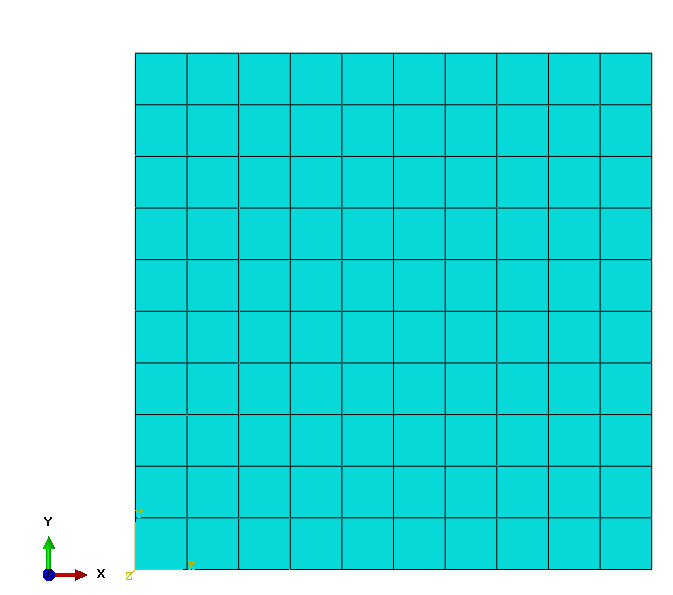
\includegraphics[width=0.40\linewidth]{images/Mesh.png}
\caption{Model discretization}
 \label{fig: Mesh}
\end{figure}

\subsection{Loading}
At the current stage, we are considering compressive or tensile loading only, with more loading scenarios envisaged in the future. Loading type is defined using text variable $ loadingType = compression $ or $loadingType = tension$. Loading direction is defined with $loading\_direction = Y$ in our example, but it could be set to X, if pressure is applied horizontally. 

A uniform pressure, measured in MPa is applied to the top of the plate as shown in \ref{fig:Load-BC}. Pressure value is given in variable $pressure = 19.5 \: MPa$.

\subsection{Boundary conditions}
The plate is supported along the bottom edge by constraining the in-plane displacements in the direction of loading (y-axis in our example). One node in the base of the plate in the transverse and out-of-plane directions (x- and z-axis, here) are also restrained for stability, as depicted in Figure \ref{fig:Load-BC}. 

\begin{figure} [H]
\centering
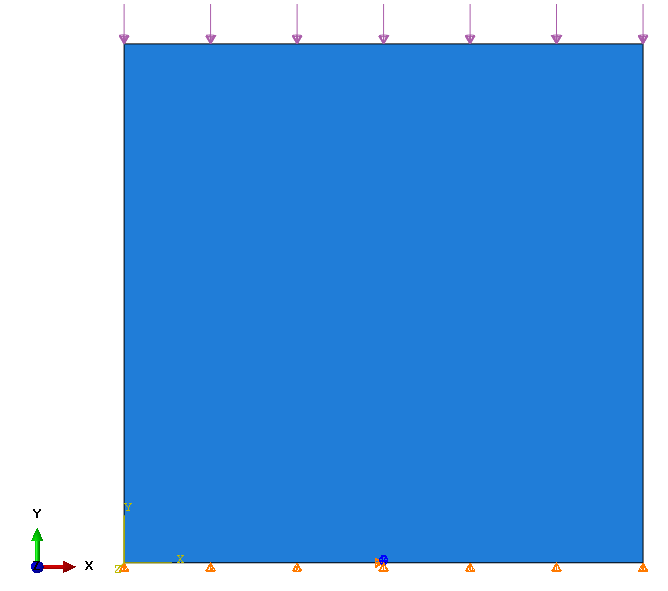
\includegraphics[width=0.40\linewidth]{images/Load_BC.png}
\caption{Model loading and boundary conditions}
 \label{fig:Load-BC}
\end{figure}

\subsection{Strain measurement}
The proposed approach requires a single strain value per element. Either an average strain or the value from the element centroid can be used. The strains shall be supplied with text files, named \textit{fileID-XXX-Eps\_xx}, \textit{fileID-XXX-Eps\_xy}, \textit{fileID-XXX-Eps\_yy}. For example \textit{fileID-012-Eps\_xx}.

The values such as strains or material properties are set throughout the mesh from the the left to right of each element row, and from the bottom to top  (see Figure \ref{fig:Elementsid}). 

\begin{figure} [H]
\centering
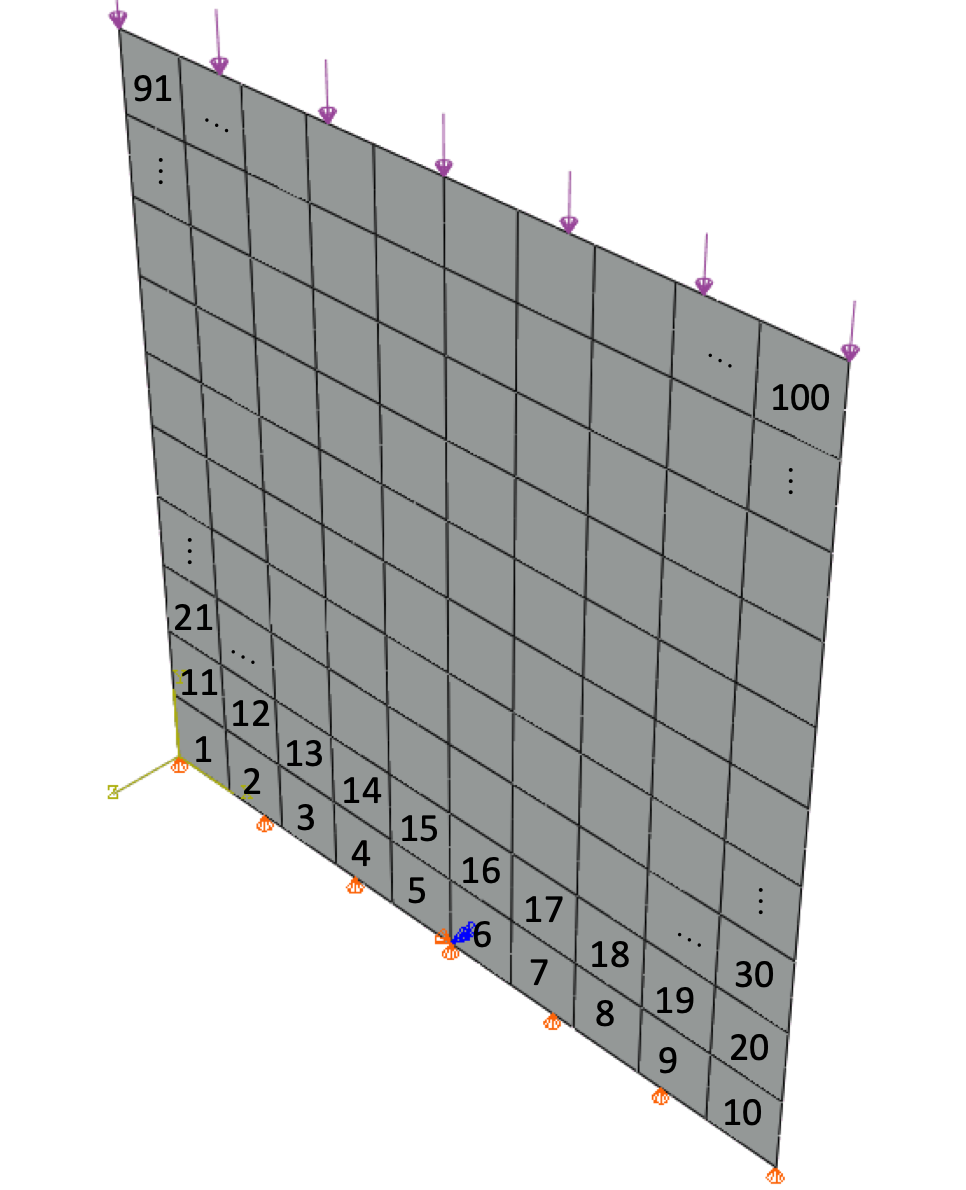
\includegraphics[width=0.40\linewidth]{images/Elements_id.png}
\caption{ Material properties distribution over the field}
 \label{fig:Elementsid}
\end{figure}

Format of the file: \\
header line: elementID, strainXX, strainYY, strainXY \\
values: 1, 0.01, 0.001, 0.001 \\
values: 1, etc.


The spatially correlated field of Young’s Modulus and Poisson’s ratio was created using mean values of 29269 MPa and 0.203, respectively.  Normal distributions were assumed for both cases.  

\section{References} 

\begin{thebibliography}{9}

\bibitem{1} http:https://classes.engineering.wustl.edu

\end{thebibliography}

\end{document}

%%
%% End of file `elsarticle-template-num.tex'.
